%%%%%%%%%%%%%%%%%%%%%%%%%%%%%%%%%%%%%%%%%%%%%%%%%%%%%%%%%%%%%%%%%%%%%%%%%%%%%%%%
\section{Information-Theoretic (IT) Proof Systems}
\label{paradigms:IT}
This section surveys various categories of 
\makebox[0pt][l]{\blue{IT proof systems}}\protect\textattachfile[mimetype={application/pdf}]{./figs/zkproof-mindmap-it-proofs-20210425.pdf}{\phantom{IT proof systems}}, designed in an idealized model.
They enable proofs that do not rely on cryptographic assumptions, often resulting in elegant and easier to understand constructions. 
Even though often these proofs cannot be used directly in the real world, they are still useful for combination with cryptographic compilers.
\loosen


%\def\extILC{Ideal Linear Commitment}  \def\ILC{\pdftooltip{ILC}{Ideal Linear Commitment}}
\def\extIOP{Interactive Oracle Proof} \def\IOP{\pdftooltip{IOP}{\extIOP}}
\def\extIP{Interactive Proof}		  \def\IP{\pdftooltip{IP}{\extIP}}
\def\extIT{Information Theoretic}	  \def\IT{\pdftooltip{IT}{\extIT}}
\def\extQAP{Quadratic Arithmetic Program} \def\QAP{\pdftooltip{QAP}{\extQAP}}
\def\extQSP{Quadratic Span Program}	  \def\QSP{\pdftooltip{QSP}{\extQAP}}
\def\extSSP{Square Span Program}	  \def\SSP{\pdftooltip{SSP}{\extSSP}}
\def\extPCP{Probabilistically Checkable Proof} \def\PCP{\pdftooltip{PCP}{\extPCP}}
\def\extMPC{[Secure] Multi-Party Computation}  \def\MPC{\pdftooltip{MPC}{[Secure] Multi-Party Computation}}
\def\extZKP{Zero-Knowledge Proof}  \def\ZKP{\pdftooltip{ZKP}{Zero-Knowledge Proof}}
\begin{figure}[!htb]
\centerline{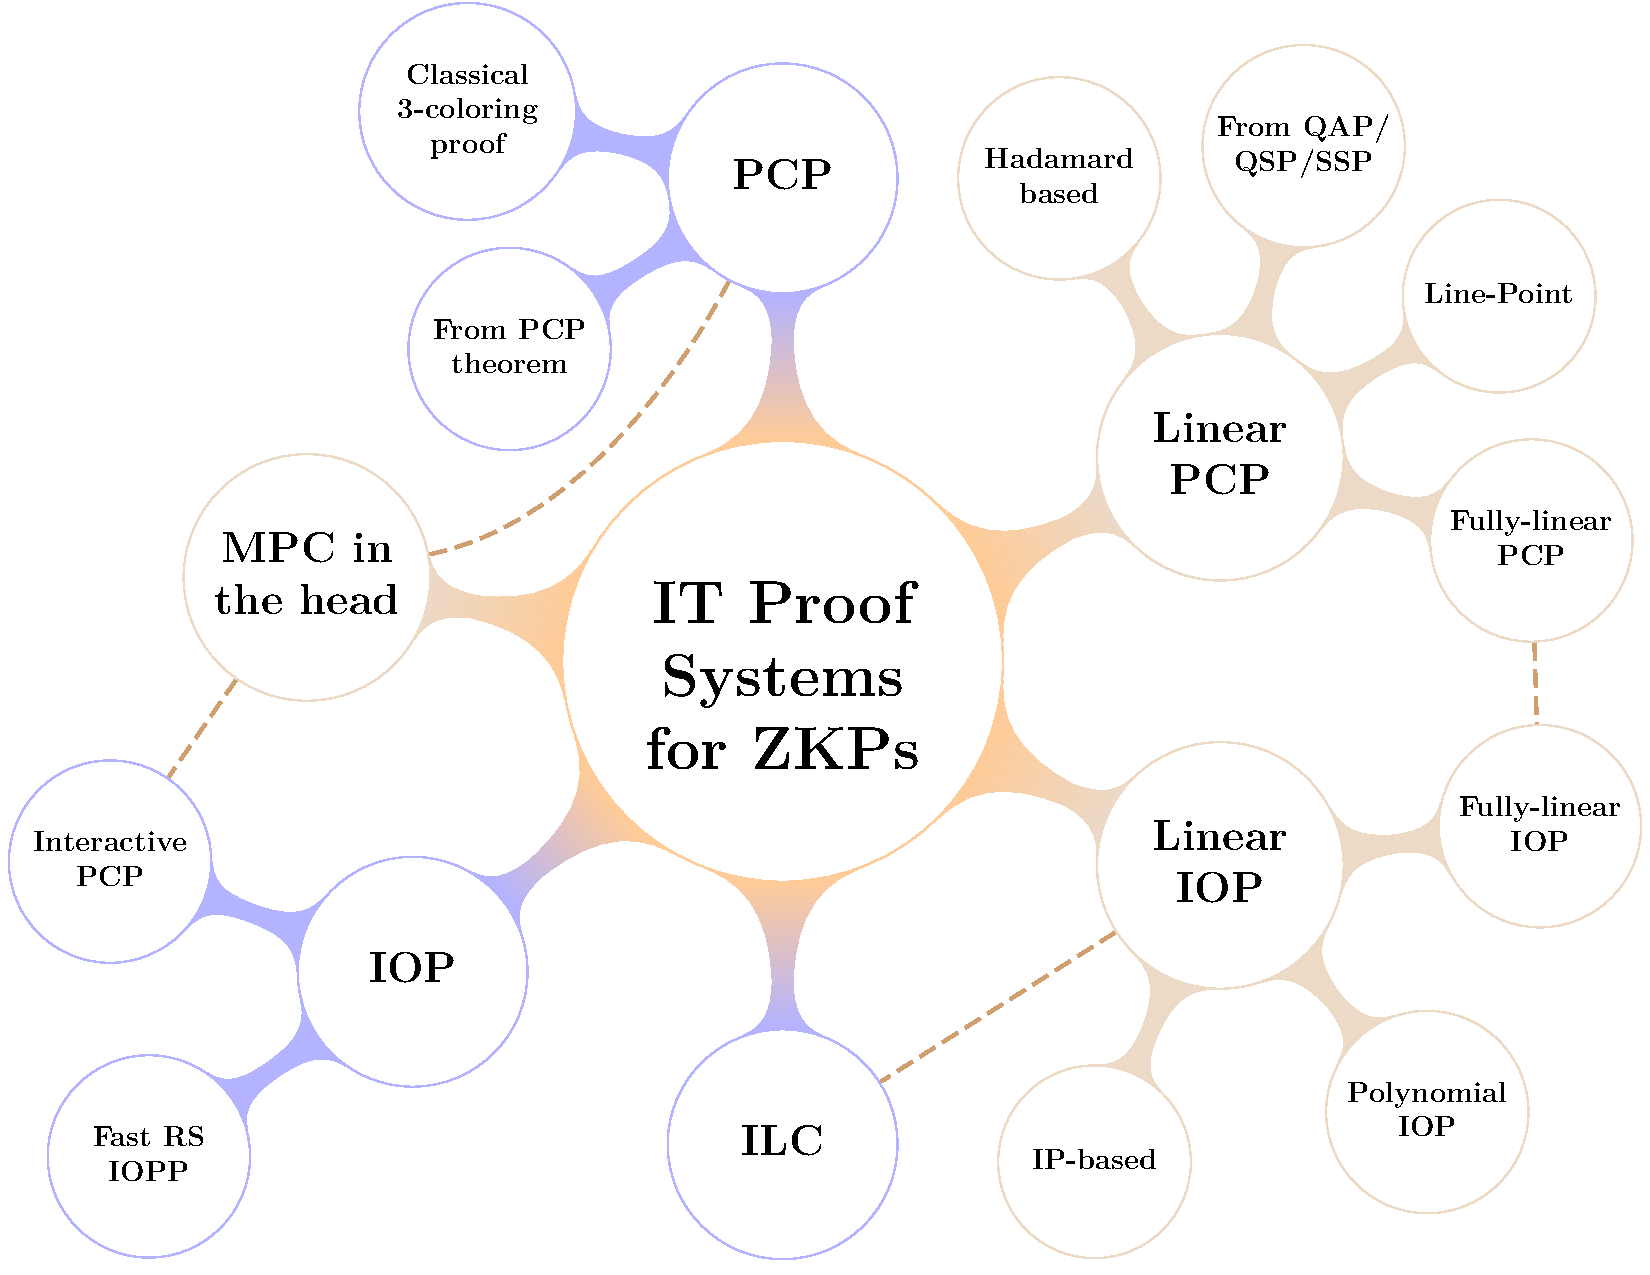
\includegraphics[width=.9\textwidth]{figs/mindmap-IT-proof-systems.pdf}} %width tailored to fit subsequent paragraph
\vskip0pt
\vspace{1.5em}
\restoline{\begin{minipage}[t]{1.16\textwidth}\setlinenumbermargin{.4em}{}\conditionalinternallinenumbers
\textbf{Legend:} 
\textbf{Fast RS IOPP} (aka FRI: Fast Reed-Solomon IOP of Proximity);
\textbf{ILC} (\extILC); 
\textbf{IOP} (\extIOP); 
\textbf{IP} (\extIP);
\textbf{IT} (\extIT);
\textbf{MPC} (\extMPC); 
\textbf{PCP} (\extPCP); 
\textbf{QAP} (\extQAP); 
\textbf{QSP} (\extQSP); 
\textbf{SSP} (\extSSP); 
\textbf{ZKP} (\extZKP).
\end{minipage}}

\caption{\label{fig:it-mindmap}Various IT proof systems}
\label{fig:IT}
\end{figure}

%%% Mindmap of Information Theoretical Proof systems, useful for ZKP paradigms
%%% Luis Brandao: initial latex code 2020-Dec--2022-April
%%% Revised with Daniel Benarroch and Eran Tromer
%%% Keywords suggested by Yuval Ishai (2020-Dec)
%%% License: ZKProof @ CC-BY 4.0 --- Creative Commons Attribution 4.0 International

%%% Update LB 2022-July: hyperlinks added (will override the tooltips), line numbers added (incomplete code to control horizontal spacing per node)

\begingroup

%%% Definitions used for legend and tooltips

\def\extILC{Ideal Linear Commitment}
\def\extIOP{Interactive Oracle Proof}
\def\extIP{Interactive Proof}

\def\extIT{Information Theoretic}

\def\extQAP{Quadratic Arithmetic Program}
\def\extQSP{Quadratic Span Program}
\def\extSSP{Square Span Program}
\def\extPCP{Probabilistic Checkable Proof}
\def\extMPC{[Secure] Multi-Party Computation}
\def\extVOLE{Vector Oblivious Linear Evaluation}
\def\extZKP{Zero-Knowledge Proof}


%%% Styles for various levels os nodes
\newcommand{\styA}[1]{\scalebox{4}{\textbf{\subtab{#1}}}}
\newcommand{\styB}[1]{\scalebox{2.75}{\textbf{\subtab{#1}}}}
\newcommand{\styC}[1]{\scalebox{2}{\textbf{\subtab{#1}}}}
\newcommand{\styD}[1]{\scalebox{1.5}{\textbf{\subtab{#1}}}}


%\renewcommand{\pdftooltip}[2]{#1}

\let\hyperrefA\hyperref
\newcommand{\hyperrefB}[2][]{#2}


%%% Central node
\def\ZKP{\pdftooltip{ZKP}{Zero-Knowledge Proof}}
\def\ITproofs{\styA{\rule{0em}{1.5em}\hyperrefA[paradigms:IT]{\subtab{\pdftooltip{IT}{\extIT} Proof\\Systems}}\\for \ZKP{}s}}


%%% 1st order nodes
\def\ILC{\styB{\pdftooltip{\hyperrefA[paradigms:IT:ILC]{ILC}}{Ideal Linear Commitment}}}
\def\IOP{\styB{\pdftooltip{\hyperrefA[paradigms:IT:IOP]{IOP}}{\extIOP}}}
\def\LIOP{\styB{\pdftooltip{\hyperrefA[paradigms:IT:linear-IOP]{\subtab{Linear\\IOP}}}{Linear \extIOP}}}
\def\PCP{\styB{\pdftooltip{\hyperrefA[paradigms:IT:PCP]{PCP}}{\extPCP}}}
\def\LPCP{\styB{\pdftooltip{\hyperrefA[paradigms:IT:linear-PCP]{\subtab{Linear\\PCP}}}{Linear \extPCP}}}
\def\MiTH{\styB{\pdftooltip{\hyperrefA[paradigms:IT:MPC-in-the-head]{\subtab{MPC in\\the head}}}{[Secure] Multi-Party Computation in the Head}}}


%%% 2nd order nodes
\def\IPbased{\styC{\pdftooltip{\hyperrefA[paradigms:IT:linear-IOP:IP-based]{IP based}}{\extIP\ based}}}
\def\PolyIOP{\styC{\pdftooltip{\hyperrefA[paradigms:IT:linear-IOP:polynomial-IOP]{\subtab{Polynomial\\IOP}}}{Polynomial \extIOP}}}
\def\FLIOP{\styC{\pdftooltip{\hyperrefA[paradigms:IT:linear-IOP:fully-linear-IOP]{\subtab{Fully Linear\\IOP}}}{Fully-linear \extIOP}}}

\def\HadBased{\styC{\hyperrefA[paradigms:IT:linear-PCP:hadamard]{\subtab{Hadamard\\based}}}}
\def\LinePoint{\styC{\hyperrefA[paradigms:IT:linear-PCP:line-point]{\subtab{Line-Point}}}}
\def\FLPCP{\styC{\pdftooltip{\hyperrefA[paradigms:IT:linear-PCP:fully-linear]{\subtab{Fully Linear\\PCP}}}{Fully-linear \extPCP}}}
\def\QAP{\pdftooltip{QAP}{\extQAP}}
\def\QSP{\pdftooltip{QSP}{\extQSP}}
\def\SSP{\pdftooltip{SSP}{\extSSP}}
\def\FromQAPQSPSSP{\styC{\hyperrefA[paradigms:IT:linear-PCP:from-QAP]{\subtab{From \QAP/\\\QSP/\SSP}}}}

\def\ClassThreeCol{\styC{\hyperrefA[paradigms:IT:PCP:3-col]{\subtab{Classical\\3-coloring\\proof}}}}
\def\FromPCPTheo{\styC{\pdftooltip{\hyperrefA[paradigms:IT:PCP:from-PCP-theorem]{\subtab{From PCP\\theorem}}}{From \extPCP\ theorem}}}

\def\InterPCP{\styC{\pdftooltip{\hyperrefA[paradigms:IT:IOP:interactive-PCP]{\subtab{Interactive\\PCP}}}{Interactive \extPCP}}}
\def\FRI{\styC{\pdftooltip{\hyperrefA[paradigms:IT:IOP:fast-RS-IOPP]{\subtab{Fast RS\\IOPP}}}{Fast Reed-Solomon \extIOP\ of Proximity}}}



\newcounter{mylinenumberbeforefigure}
\setcounter{mylinenumberbeforefigure}{\value{linenumber}}
\addtocounter{mylinenumberbeforefigure}{-1}
\newcounter{cntNumLinesInFig}\setcounter{cntNumLinesInFig}{0}
\let\origthelinenumber\thelinenumber
% \setlinenumbermargin{#1}
% \renewcommand{\thelinenumber}{\hspace*{#1}\origthelinenumber}
% \renewcommand{\thelinenumber}{\makebox[0pt][l]{\value{linunumber}\hspace{#1}}}
\newlength{\myLNhorizoffset}
\setlength{\myLNhorizoffset}{-1.5em}

%%%%%%%%%%%%%%%%%%%%%%%%%%%%%%%%%%%%%%%%
\nolinenumbers
% LNO: line number ordering --- function that will (manually) inform the line number of each node
\newcommand{\LNO}[2][0pt]{\stepcounter{cntNumLinesInFig}
    \setcounter{linenumber}{\value{mylinenumberbeforefigure}}
		\addtocounter{linenumber}{#2}
    \setlength{\myLNhorizoffset}{#1}}
\begin{figure}[H]\centering  % !htb
\def\tmpfigcap{Various IT proof systems}
\refstepcounter{figure}\label{fig:it-mindmap}%
\hypertarget{ht:figure:\thefigure}{}
\addcontentsline{lof}{figure}{Figure~\thefigure{}: \tmpfigcap}
\nolinenumbers
\bookmarksetup{level=3,color=\colorbkmfig}
\bookmark[dest=ht:figure:\thefigure]{Figure~\thefigure}%

\begingroup  %% begin scope for changed \thelinenumbers
\let\tempthelinenumber\thelinenumber
\nolinenumbers


%\conditionalinternallinenumbers
%https://tex.stackexchange.com/questions/281226/tikz-getting-angles-in-mindmaps-right
\tikzset{grow cyclic list/.code={%
  \def\tikzgrowthpositions{{#1}}%
  \foreach \n [count=\i,remember=\i]in {#1}{}%
  \let\tikzgrowthpositionscount=\i%
  \tikzset{growth function=\tikzgrowcycliclist}}}
\def\tikzgrowcycliclist{%
  \pgftransformshift{%
    \pgfpointpolar{\tikzgrowthpositions[mod(\the\tikznumberofcurrentchild-1,\tikzgrowthpositionscount)]}%
      {\the\tikzleveldistance}}}

\makeatletter\tikzset{concept/.style={circle,draw=\tikz@concept@color,every concept}}\makeatother%
\centering%


% https://tikz.dev/tikz-shapes#section-nodes-multi
\vspace{1em}
%%%\centerline{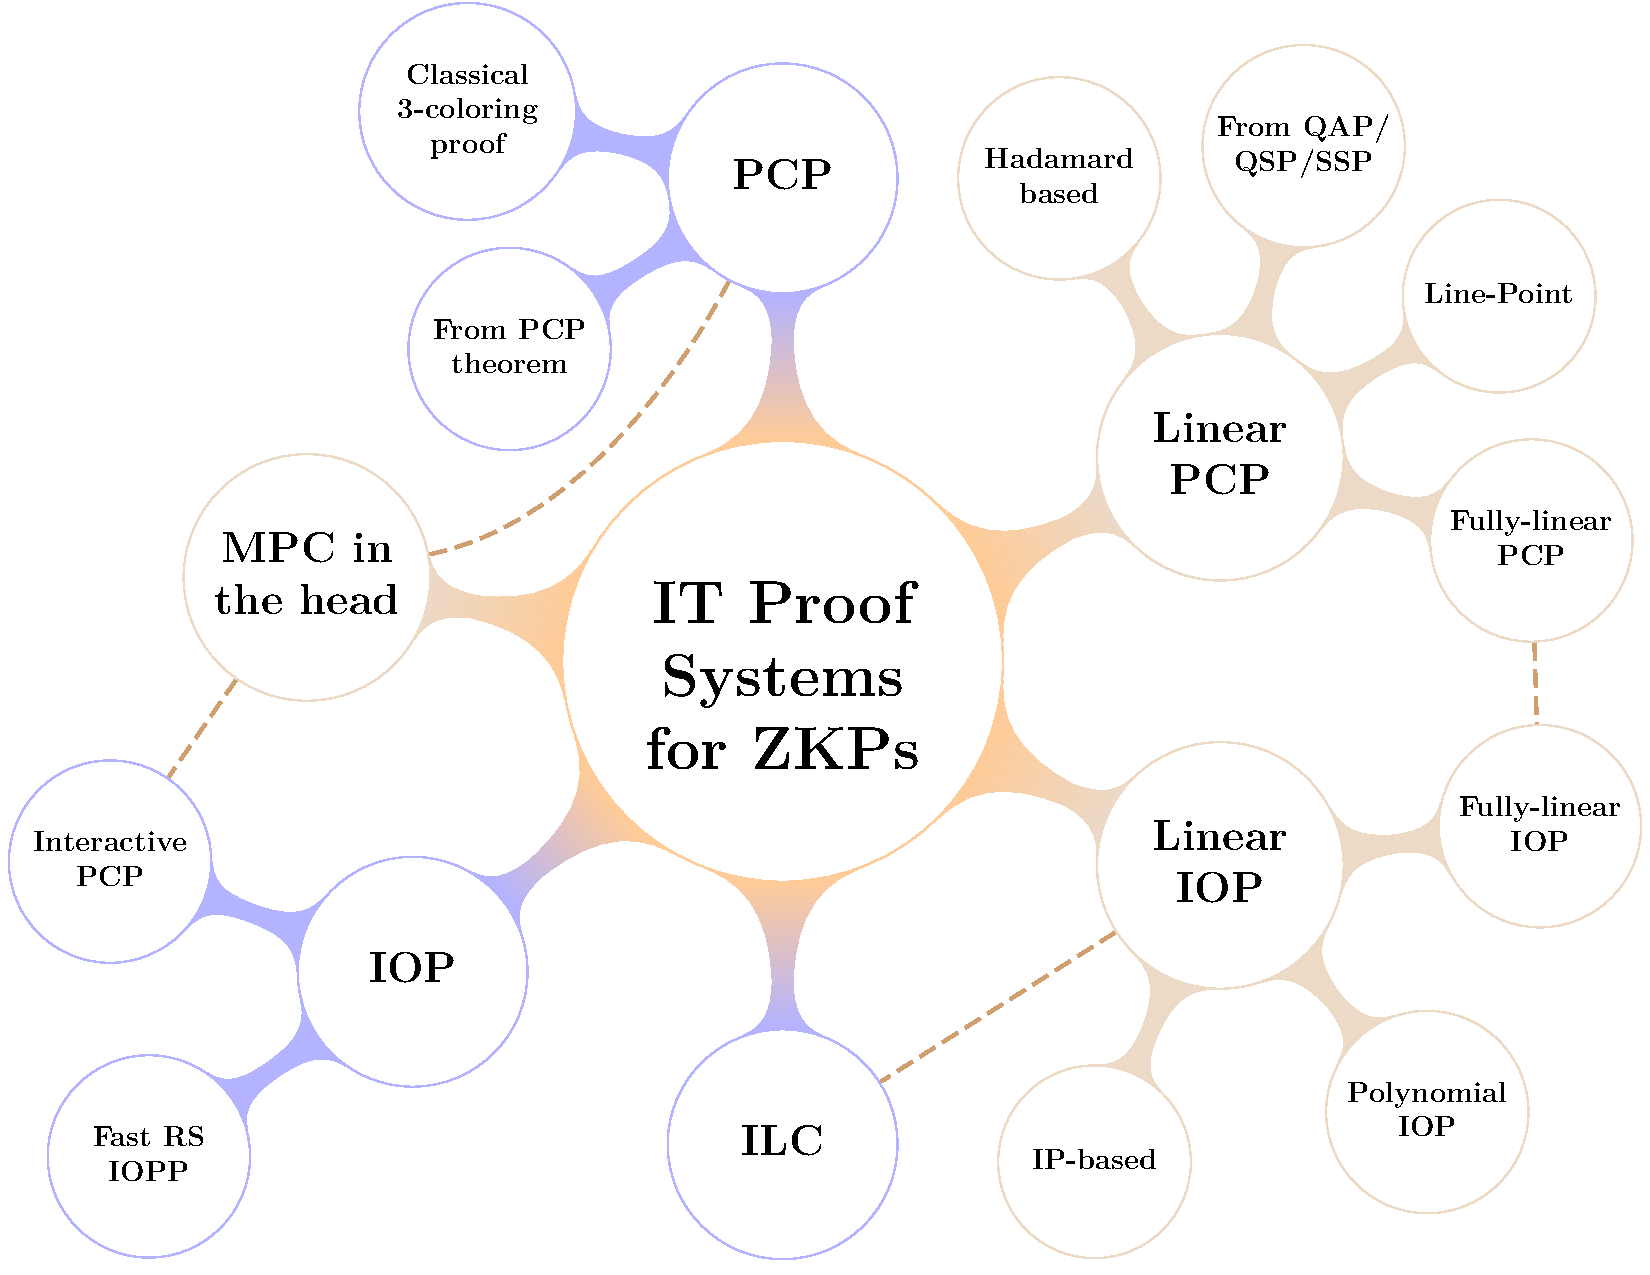
\includegraphics[width=.9\textwidth]{figs/mindmap-IT-proof-systems.pdf}} %width tailored to fit subsequent paragraph
\resizebox{.95\textwidth}{!}{\begin{tikzpicture}[rotate=+90,
execute at begin node = {\conditionalinternallinenumbers\renewcommand{\thelinenumber}{\scalebox{3}{\makebox[0pt][l]{\hspace*{\myLNhorizoffset}\tempthelinenumber}}}}
]     %%% if including legend and having margins .5in
\path[mindmap, grow cyclic, text width=4.4in, every node/.style=concept, align=flush center, concept color=orange!40, fill={none},
			%/.append style
			level 1/.style={text width=2.75in, level distance=6in, sibling angle=90, fill={none}},  
			level 2/.style={text width=2.33in, level distance=4.0in, sibling angle=45, fill={none}},
			level 3/.style={text width=1.15in, level distance=2.75in, sibling angle=45, fill={none}},
			%https://tex.stackexchange.com/questions/145991/inserting-special-border-to-tikz-mindmap
			marca/.append style={fill={none}}, outer sep=1pt
			]

%\setlength{\myLNhorizoffset}{-2.5em}
%node[concept, append after command=\pgfextra{\setlength{\myLNhorizoffset}{-5em}}] {\LNO[4em]{10}\ITproofs} %% \LNO[-1em]{10}
node[concept] {\LNO[4em]{10}\ITproofs} %% \LNO[-1em]{10}
%%%%
child[grow=0, concept color=blue!30] { node (pcp) {\LNO{3}\PCP} %%% \setlength{\myLNhorizoffset}{-1.5em}
	child[grow=78] { node {\LNO{1}\ClassThreeCol}}
	child[grow=122] { node {\LNO{6}\FromPCPTheo}}  %\zk-\PCP\\
}
child[grow=80, concept color=brown!30] { node (mpchead) {\LNO{9}\MiTH}
}
child[grow=130, concept color=blue!30] { node (iop) {\LNO{14}\IOP}
	child[grow=70] { node (interactivepcp) {\LNO{12}\InterPCP}}
	child[grow=125] { node {\LNO{17}\FRI}}
}
child[grow=180, concept color=blue!30] { node (ilc) {\LNO{16}\ILC}
}
child[grow=245, concept color=brown!30] { node (lineariop) {\LNO{13}\LIOP}    %color=teal!30
	child[grow=277] { node (FLIOP) {\LNO{11}\FLIOP}}
	child[grow=220.5] { node {\LNO{15}\PolyIOP}}
	child[grow=157] { node {\LNO{18}\IPbased}}
}
child[grow=-65, marca, concept color=brown!30] { node {\LNO{7}\LPCP} 
	child[grow=30] { node {\LNO{4}\HadBased}}
	child[grow=-15] { node {\LNO{2}\FromQAPQSPSSP}}
	child[grow=-60] { node {\LNO{5}\LinePoint}}
	child[grow=-105] { node (FLPCP) {\LNO{8}\FLPCP}}
};


%%% https://tex.stackexchange.com/questions/266983/adding-an-independent-small-node-in-a-mind-map
\begin{pgfonlayer}{background}
    %\draw [left color=blue, right color=green!50!black, draw=white, decorate,decoration=circle connection bar] (mpchead) -- (pcp);
	\draw[dash pattern=on 16pt off 8pt,line width=3pt, brown!75] (mpchead) to[out=-50,in=180] (pcp);
    \draw[dash pattern=on 16pt off 8pt,line width=3pt, brown!75] (mpchead) -- (interactivepcp);
    \draw[dash pattern=on 16pt off 8pt,line width=3pt, brown!75] (FLPCP) -- (FLIOP);
	\draw[dash pattern=on 16pt off 8pt,line width=3pt, brown!75] (lineariop) -- (ilc);  %to[out=160,in=-20]

\end{pgfonlayer}

\end{tikzpicture}
} %% end of \restoline

\endgroup  %% end scope for changed \thelinenumbers

\addtocounter{mylinenumberbeforefigure}{\value{cntNumLinesInFig}}
\setcounter{linenumber}{\value{mylinenumberbeforefigure}}
\stepcounter{linenumber}

\vskip0pt
\vspace{1.5em}
\nolinenumbers
\restoline{\begin{minipage}[t]{1.07\textwidth}\setlinenumbermargin{.4em}{}\conditionalinternallinenumbers
\textbf{Legend:} 
\textbf{Fast RS IOPP} (aka FRI: Fast Reed-Solomon IOP of Proximity);
\textbf{ILC} (\extILC); 
\textbf{IOP} (\extIOP); 
\textbf{IP} (\extIP);
\textbf{IT} (\extIT);
\textbf{MPC} (\extMPC); 
\textbf{PCP} (\extPCP); 
\textbf{QAP} (\extQAP); 
\textbf{QSP} (\extQSP); 
\textbf{SSP} (\extSSP); 
\textbf{ZKP} (Zero-Knowledge Proof).
\end{minipage}}

\conditionalinternallinenumbers % to get line number in caption of figure
\vskip.75em\textbf{Figure \thefigure. }\tmpfigcap
%%% \caption{\label{fig:it-mindmap}}
\end{figure}

\endgroup


\linenumbers



\paragraph{Notation} 
A verifier is said to make ``point queries'' to the proof $\Pi$ if the verifier has access to a proof oracle $O^{\Pi}$ that takes as input an index $i$ and outputs the $i$-th symbol $\Pi(i)$ of the proof. 
A verifier is said to make ``inner-product queries'' to the proof $\Pi \in \field^m$ (for some finite field \field) if the proof oracle takes as input a vector $q \in \field^m$ and returns the value $\brktmath{\Pi, q} \in \field$. 
A verifier is said to make ``matrix-vector queries'' to the proof $\Pi \in \field^{m\times k}$ if the proof oracle takes as input a vector $q \in \field^k$ and returns the matrix-vector product $(\Pi.q) \in \field^m$.


%%%%%%%%%%%%%%%%%%%%%%%%%%%%%%%%%%%%%%%%%%%%%%%%%%%%%%%%%%%%
\subsection{Summary}
\label{paradigms:taxonomy:proof-systems}


In a classical proof of a statement $x$, the prover sends a proof string $\pi$ for complete reading by the verifier, who then \emph{accepts} if and only if the proof conveys an efficient absolute-verifiability of the statement's truth.
For example, a trivial (not ZK) example of \emph{classical} proof of knowledge is the direct sending of the known witness $w$.

The field of proof checking has meanwhile evolved to encompass interactive proofs (where the convincing comes from an interaction, rather than from the analysis of a sole string) and arguments (where certainty is not absolute, but still overwhelming), and often with a ZK feature.
\loosen


This section explains IT proof systems that often make use of ideal (unrealizable) components and are not necessarily ZK, but which allow for a later compilation of real proofs that are both succinct and ZK.  
\reffigure{fig:it-mindmap} considers the following main types of IT proof systems:
\loosen
    
    %%% EDITORIAL NOTE: REFRAIN FROM CITATIONS IN THIS SUMMARIZED ENUMERATION. 
    %%% CITATIONS ARE LEFT FOR THE SUBSEQUENT SUBSECTIONS AND SECTIONS.

	\begin{enumerate}[label=\alph*.]
  
	\item\pslabel{proof-system:classical-PCP}
	\textbf{\hyperref[paradigms:IT:PCP]{Probabilistically Checkable Proof (PCP)}}: 
	In a PCP proof, the prover sends the verifier a (possibly very long) proof string $\pi$; the verifier makes ``point queries'' to the proof, reads the entire statement x, and accepts or rejects. 
  
	\item\pslabel{proof-system:linear-PCP} 
	\textbf{\hyperref[paradigms:IT:linear-PCP]{Linear PCP}:} 
	In a linear PCP proof, the prover sends the verifier a (possibly very long) proof string $\pi$, lying in a vector space $\F^m$. 
	The verifier makes a number of linear queries to the proof, reads the entire statement $x$, and accepts or rejects. 
	\loosen
  
    \item\pslabel{proof-system:mpc-in-the-head}
    \textbf{\hyperref[paradigms:IT:MPC-in-the-head]{MPC-in-the-head}:}
    A proof can be composed of the partial views of a simulated security multi-party computation (MPC) execution with semi-honest security.
    The witness is secret-shared between the simulated parties, who then (by simulation) securely compute the ZKP predicate.
    The partial transcript simultaneously ensures soundness and ZK.\loosen
  
	\item\pslabel{proof-system:IOP} 
	\textbf{\hyperref[paradigms:IT:IOP]{Interactive Oracle Proof (IOP)}:} 
	An IOP is a generalization of a PCP, to consider the interactive setting. 
	In each round of communication, the verifier sends a challenge string $c_i$ to the prover, and then the prover responds with a PCP proof $\pi_i$, which the verifier may query via point queries.
	After several rounds of interactions, the verifier accepts or rejects.

  
	\item\pslabel{proof-system:linear-IOP} 
	\textbf{\hyperref[paradigms:IT:linear-IOP]{Linear IOP}:} 
	A linear IOP is a generalization of a linear PCP to the interactive setting. (See IOP above.) 
	Here the prover sends in each round a proof vector $\pi_i$ that the verifier may query via linear (inner-product) queries.
  
	\item\pslabel{proof-system:ILC} 
	\textbf{\hyperref[paradigms:IT:ILC]{Ideal Linear Commitment (ILC)}:} 
	The ILC model is similar to linear IOP, except that in each round the prover sends a proof matrix rather than a proof vector; the verifier learns the product of the proof matrix and the query vector. 
	Each ILC proof matrix may be the output of an arbitrary function of the input and the verifier's messages, not limited to linear functions.

	\end{enumerate}


\futfig{One table of figures, pictorially comparing the various IT proof systems}


%%%%%%%%%%%%%%%%%%%%%%%%%%%%%%%%%%%%%%%%%%%%%%%%%%%%%%%%%%%%
\subsection{Probabilistically Checkable Proof (PCP)}
\label{paradigms:IT:PCP}

A probabilistically checkable proof is a proving paradigm that assumes an interaction between the prover and the verifier.
The prover sends a first message and can only convince the verifier in later messages if there exists a valid witness.
In this section we first present a classic PCP example for proving the $3$-coloring problem.
Then we provide a more precise explanation of the PCP information theoretic paradigm and the PCP theorem.


%%%%%%%%%%%%%%%%%%%%%%%%%%%%%%%%%%%%%%%%%
\subsubsection{Classical 3-coloring proof}\label{sec:3coloring}
\label{paradigms:IT:PCP:3-col}


The graph 3-coloring problem was the basis for the first ZKP system for NP \cite{1991:GMW:JACM:proofs-that-yield-nothing-but-their-validity}.
The \emph{instance} of the problem is an undirected graph $G=(V,E)$.
The \emph{statement} (i.e., the goal of what to prove) is that the graph has a 3-coloring, i.e., that each node $i \in V$ (in the set $V$ of vertices) can be assigned one of three colors $c(i) \in \{1,2,3\}$, such that any edge $(i,j) \in E$ (i.e., any pair of connected nodes) connects two vertices with distinct colors.
The \emph{witness} is a coloring assignment $c:V\to\{1,2,3\}$, mapping each node to one of three colors.


Let $R_{\sf 3COL}$ denote the \emph{relation} of interest, used to test whether $c$ is a good 3-coloring for a given graph $G$, i.e., satisfying $(G,c)\in R_{\sf 3COL} \Leftrightarrow \#(c) = 3 \wedge ~c(u)\neq  c(v)$ for every $(u,v)\in E$.
Since the relation $R_{\sf 3COL}$ is {\em NP-complete}, having a ZKP for proving that a graph is 3-colorable implies having a ZKP for proving membership in any other NP language (say, associated with a relation $R$).
This is done by having the prover and the verifier locally apply a polynomial-time reduction to convert their inputs for $R$ into inputs for $R_{\sf 3COL}$. 


%%%%%%%%%%%%%%%%
\paragraph{The protocol}
The classical ZKP for $R_{\sf 3COL}$ proceeds as follows. 
(Here we consider an IT system that provides an ideal commitment functionality.)

\begin{itemize}
\item The prover, on input $(G,c)$, picks a random permutation $\phi:\{1,2,3\}\to\{1,2,3\}$ defining a random shuffle of the colors, and lets $c'(v)=c(\phi(v))$ be the shuffled coloring. 

\item For each node $v \in V$, the prover commits to the shuffled color $c'(v)$. (In the real world the prover sends (or interacts, in order to provide) a commitment to the verifier.)
\loosen

\item The verifier asks the prover to open the colors of a uniformly selected edge $(u,v)\in E$.

\item The prover opens the commitments, revealing $c'(u)$ and $c'(v)$ to the verifier.

\item The verifier accepts $G$ (as a 3-colorable graph) iff the prover successfully opens the two commitments and they contain different values in $\{1,2,3\}$. 
\end{itemize}


\futfig{Illustrate the classical R3Col ZKP protocol}


%%%%%%%%%%%%%%%%
\paragraph{Security analysis}
The above protocol satisfies the three needed properties:

\begin{itemize}
\item \textbf{Completeness:} if the coloring $c$ is valid then so is its permuted version $c'$, and so an honest prover will always successfully open two distinct colors in $c'$. 
 
\item \textbf{ZK:} only the two shuffled colors $(c'(u),c'(v))$ are revealed, but they could be \emph{simulated} (see \refsec{sec:security:defs-props:zero-knowledge}) by choosing any random pair of {\em distinct} colors. 
This holds even for a malicious verifier that chooses $u$ and $v$ arbitrarily, as long as the prover checks they form a valid edge.\loosen

\item \textbf{Soundness:}
if $G$ does not admit a valid coloring, then no matter which colors $c^*$ are committed to by a malicious prover, there is at least one edge $(u,v)\in E$ that will satisfy $c^*(u)=c^*(v)$. 
Therefore, the verifier will reject the proof with at least $1/|E|$ probability. 
This poor level of soundness can be amplified, while preserving zero knowledge, by sequentially running the protocol many times independently  (e.g., $\kappa\cdot|E|$ for an error probability or about $2.7^{-k}$).  
Note that a parallel repetition would not preserve ZK.

\end{itemize}


%%%%%%%%%%%%%%%%%%%%%%%%%%%%%%%%%%%%%%%%%
\subsubsection{From PCP theorem}
\label{paradigms:IT:PCP:from-PCP-theorem}

In general, in a PCP for an NP-relation $R$, the prover computes a probabilistic polynomial-time mapping from a statement-witness pair $(x,w)$ to a proof string $\pi\in\Sigma^m$ (i.e., a string of length $m$ over some finite alphabet $\Sigma$). The verifier queries a randomly chosen subset of the symbols of $\pi$, and then decides whether to accept or reject.
Crucially, the content of $\pi$ is produced by the prover without knowing which indices into $\pi$ will be queried by the verifier.
More precisely, the verifier's algorithm is specified by a randomized mapping from an instance $x$ to a subset $Q\subset[m]$ of queried symbols, and a decision predicate $D(x,Q,\pi_Q)$ deciding whether to accept or reject based on the contents of the queried symbols. 
The PCP theorem \cite{2000:SIAM:Computationally-Sound-Proofs,1992:kilian:note-on-efficient-ZKPs-and-args} roughly states the following.

\begin{theorem}[The PCP Theorem]\label{thm:pcp}
    For all languages in $NP$ there exists an efficient PCP with logarithmic communication complexity.
\end{theorem}

A \emph{zero-knowledge PCP} (zk-PCP) moreover fulfills the zero-knowledge property (see \refsec{sec:security:defs-props:zero-knowledge}), where the zero-knowledge simulator is required by default to {\em perfectly} sample the view $(Q,\pi_Q)$ of an {\em honest} verifier given $x$ alone.
We assume that one can efficiently recognize whether a set $Q$ can be generated by an honest verifier on a given input $x$.
In the literature non-zk PCPs are often required to have small query complexity but see that the three coloring example is zero-knowledge and not small query complexity.


%%%%%%%%%%%%%%%%
\paragraph{Example: 3-coloring as a PCP}
In the 3-coloring example of \cref{sec:3coloring} above, $\pi$ is a string of length $m=|V|$ over $\Sigma=\{1,2,3\}$ comprised of the values $c'(v)$ for $v\in V$, where the randomness is over the permutation $\phi$ used to convert $c$ into $c'$.
Here, $Q$ is uniformly distributed over sets of size 2 corresponding to edges in $E$, and $D$ accepts if the two queried symbols are distinct.
The basic version of the zk-PCP for $R_{\sf 3COL}$ has a high soundness error of $1-1/|E|$.
Soundness can be amplified, while respecting (honest verifier) zero knowledge, by concatenating independently generated proofs $\pi^{(i)}$ and querying them independently. Note that making multiple queries to the {\em same} $\pi$ would compromise zero knowledge.


\paragraph{Discussion}
The above notion of zk-PCP is information-theoretic in the sense that both soundness and (honest-verifier) zero knowledge hold with respect to computationally unbounded parties.
The reason it cannot be {\em directly} used as a zero-knowledge proof protocol, without additional cryptographic machinery, is that it is not clear how to only allow the verifier a restricted access to $\pi$, which is necessary for zero knowledge, without allowing a malicious prover to violate the independence assumption between $\pi$ and $Q$ on which soundness relies.
Put differently, if $Q$ is sent to the prover first, then a malicious prover can violate soundness, and if $\pi$ is sent to the verifier in its entirety, then zero knowledge is compromised even when the verifier is honest.
The role of a cryptographic compiler is to convert an arbitrary zk-PCP (possibly with some syntactic restrictions) into a zero-knowledge proof protocol. 
\loosen


%%%%%%%%%%%%%%%%%%%%%%%%%%%%%%%%%%%%%%%%%%%%%%%%%%%%%%%%%%%%
\subsection{Linear PCP}
\label{paradigms:IT:linear-PCP}

The PCP model and the associated PCP theorem are surprisingly powerful, but entail a high cost: the prover needs to explicitly write out a long proof, most of which will not be read.
This cost can be reduced by changing the idealized model to allow a different and more expressive kinds of queries.
Intuitively, the prover will produce a small proof, which can be queried via a much larger query space, so the query procedure undertakes some of the burden. 
\loosen

\futfig{Illustrate a generic linear PCP}

A simple and useful instance of this is the {\em linear PCP} (LPCP) model.
Whereas in a standard PCP the verifier is allowed to make a bounded number of {\em point queries}, which read individual symbols of the proof $\pi$, a {\em linear PCP} allows each query to take an arbitrary linear combination of the entries of $\pi$.
More concretely, in a linear PCP over a finite field $\F$ the proof is a vector $\pi\in\F^m$ and each query $q_i\in\F^m$ returns the inner product $\langle \pi,q_i\rangle$.
We require by default that the queries $q_i$ be {\em input-oblivious}, in the sense that they can be picked independently of $x$.
One can construct such an LPCP for any NP-relation $R$ with polynomial proof size $m$,  soundness error $O(1/|\F|)$, and a constant number of queries.
The main price we pay for the more powerful PCP model is that the corresponding cryptographic compilers typically need to rely on stronger primitives that live in the ``public-key cryptography'' world, and moreover require strong forms of setup to fully respect the efficiency features of the underlying LPCP.

LPCPs were introduced as a way to achieve simple low-communication proof systems \cite{2007:IKO}.
An initial motivation was to replace complex PCP machinery by simpler one, at the cost of using stronger cryptography.

However, it was already observed back then that beyond simplicity,  this new approach can lead to an efficiency feature that was not possible via the traditional PCP-based approach: 
prover-to-verifier communication that includes only a constant number of ``ciphertexts,'' or group elements, independently of the complexity of $R$.

Below we describe two types of linear PCP: Hadamard-based and Quadratic Arithmetic Programs (QAP).
These are the most commonly used linear PCPs in the current literature.
Other types of linear PCP exist which are not discussed in this document, including Quadratic Span Programs (QSP), Square Span Programs (SSP), and Line Point based.


%%%%%%%%%%%%%%%%%%%%%%%%%%%%%%%%%%%%%%%%%
\subsubsection{Hadamard based}
\label{paradigms:IT:linear-PCP:hadamard}
To present the Hadamard-based LPCP, it is convenient to consider the NP-relation as an arithmetic circuit over a finite field $\F$, whose gates perform field additions and multiplications. Concretely, the prover wants to convince the verifier that there is a witness $w\in\F^m$ such that $C(x,w)=0$, where $C$ is a publicly known arithmetic circuit and $x\in\F^n$ is the public statement. 
\loosen

\xetexfontscale{.99}{
$C$ and $x$ are first converted into a system of $s$ {\em quadratic} equations of the form $Q_i(Y)=0$, where each $Q_i$ is a multivariate polynomial of degree (at most) 2 in $s$ variables $Y_1,\ldots,Y_s$, such that there is a $w\in\F^m$ satisfying $C(x,w)=0$ if and only if there is a $y\in\F^s$ satisfying $Q_i(y)=0$ for all $i$. 
}

In a Hadamard LPCP for proving the satisfiability of $Q_i(Y)$, the prover, on input $(x,w)$, first computes the values $y\in\F^s$ of all $s$ gates of $C$ on input $(x,w)$. 
Then it computes a quadratic sized vector $\hat{y} \in \F^{s^2}$ of entries $\hat{y}_{j k} = y_j y_k$, and outputs the proof $\pi=(y, \hat y)$.
Note that every degree-2 polynomial in $y$ can be obtained by the verifier by making a single linear query to $\pi$.

The verifier's queries achieve two goals: (1) check consistency of the two parts of $\pi$ with the tensoring relation; (2) check satisfiability of all $Q_i$ relations.  Goal (1) is realized by comparing two different ways of computing a {\em random} linear combination  $\left(\Sigma_{j=1}^s r_jy_j\right)^2$ of the entries of $y$: first by querying directly, and second by querying for the corresponding combination of $r_j r_k y_j y_k$.
Goal (2) is realized by querying for $Q_i(y)$ and verifying that $Q_i(y) = 0$. 
Soundness follows from the Schwartz-Zippel Lemma \cite{2010:Mosh}. 


%%%%%%%%%%%%%%%%
\paragraph{Fast verification}
The first feature is {\em fast verification} given input-independent preprocessing.
Whereas the cost of generating the queries $q_i$ grows with the size of the verification circuit $C$, the verifier can generate the queries before the input $x$ is known and only keep $r_1,\ldots,r_n$ for later use. 
Once $x$ is known, the verifier can compute  $\alpha=\sum_{i=1}^n r_i x_i$, using only $O(n)$ arithmetic operations. 
Finally, once the LPCP answers $a_1,a_2,a_3$ are available, the verifier can decide whether to accept by checking that $a_2=a_1^2$ and $a_3=\alpha$, which only takes $O(1)$ field operations. 
This fast verification feature is particularly useful when the same queries are reused for proving multiple statements.


\xetexfontscale{.99}{
\paragraph{Reusable soundness}
Another feature of the Hadamard LPCP is a strong form of soundness that holds even when the same queries are reused for verifying multiple proofs: 
for any $x$ and proof $\pi^*$, the prover can predict based on $x,\pi^*$ alone whether the verifier will accept, except with $O(1/|\F|)$ error probability (over the verifier's unknown random queries). 
This means that when $\F$ is sufficiently big (say, $|\F|\ge 2^{80}$), learning whether the verifier accepted $\pi^*$ reveals only a negligible amount of information about the queries $q_j$.  
The latter strong soundness property is useful for making the SRS in LPCP-based SNARGs reusable even when the prover can learn whether the verifier accepted each instance. 
This is contrasted with classical (zk-)PCPs, which are inherently susceptible \cite{2019:CDIKLOV:reusable-NISC} to a ``selective failure'' attack in which a malicious prover can gradually learn the secret set of queries when it is reused for multiple proofs. 
This can be done by slightly perturbing honestly generated proofs and learning whether the verifier accepted each perturbed proof instance. 
}

%%%%%%%%%%%%%%%%%%%%%%%%%%%%%%%%%%%%%%%%%
\subsubsection{From QAP (R1CS)}
\label{paradigms:IT:linear-PCP:from-QAP}

Colloquially, constraint systems are often called ``circuits'', but they can also take forms different from Boolean and arithmetic circuits.
While some schemes compile arithmetic circuits into zero-knowledge proofs directly \cite{1998:crypto:zkps-for-finite-field-arithmetic} it is sometimes more convenient to work with quadratic arithmetic programs (QAP).  QAPs are \emph{bilinear constraint systems} (BCS) over finite fields where each constraint allows a quadratic combination of two inputs.
That is, multiplication by scalar, addition and multiplication.

To be precise, the BCS considered here is the same as the ``system of rank-1 quadratic equations'' defined in \cite[Appendix~E]{2013:BCGTV:crypto:SNARKs-for-C}, with a minor change in notation. 
Here, $\vwit$ denotes just the witness; whereas, in the latter, $\mathbf{w}$ denotes the concatenation of the instance and the witness (and thus added corresponding consistency checks between $\mathbf{w}$ and the instance $\mathbf{x}$). 

\xetexfontscale{.99}{These are also essentially identical to the ``Rank 1 Constraint System (R1CS)'' of libsnark \cite{libsnark}.
An equivalent formulation can expressed as quadratic arithmetic programs (following \cite{2013:GGPR:eurocrypt:QSPs-and-succinct-NIZKs-without-PCPs,2013:PHGR:SP:Pinocchio,2013:BCGTV:crypto:SNARKs-for-C,BCTV13von} and others), directly reasoning about polynomial divisibility.}


A bilinear constraint system reasons about two vectors: 
the \emph{instance} consisting of $n_{\mathsf{x}}$ elements and denoted $\overrightarrow{x}=(x_1,\ldots,\NumInst)$, 
and the \emph{witness} consisting of \NumWit\ elements and denoted $\overrightarrow{w}=(w_1,\ldots,w_{\NumWit})$. 
The constraint system says that the two are related by some number of constraints, $\NumConstr$.
each of which is a quadratic equation of a specific form. All of the elements and operations are over a large prime field $\mathbb{F}_p$, which we will represent here as the integers modulo a large prime $p$.
The specific prime, and the representation of field elements, are related to the elliptic curve used in the QAP-based zkSNARK constructions.


\vskip1em\begin{definition}
\label{def:bcs}
Let $\NumInst,\NumWit,\NumConstr$ be positive integers, and $\NumConc=\NumInst+\NumWit+1$.
A \emph{bilinear constraint system} over $\Field$ is a tuple
$\System = \big((\vec{\lcoef}_{j},\vec{\rcoef}_{j},\vec{\ocoef}_{j})_{j=1}^{\NumConstr},\NumInst\big)$
where $\vec{\lcoef}_{j},\vec{\rcoef}_{j},\vec{\ocoef}_{j} \in \Field^{\NumConc}$.
Such a system $\System$ is \defem{satisfiable} with an input $\vinst \in \Field^{\NumInst}$ if the following is true:

\NPstatement
  {For these
    $\System = \big((\vec{\lcoef}_{j},\vec{\rcoef}_{j},\vec{\ocoef}_{j})_{j=1}^{\NumConstr},\NumInst\big)$
   and $\vinst \in \Field^{\NumInst}$}
  {there exists a witness $\vwit \in \Field^{\NumWit}$}
  {such that
  $\bigip{\vec{\lcoef}_{j}}{\vconc} \cdot \bigip{\vec{\rcoef}_{j}}{\vconc}  = \bigip{\vec{\ocoef}_{j}}{\vconc}$ \hskip0.4em for all for $j \in [\NumConstr]$, where $\vconc=(1,\vinst,\vwit)\in \Field^{\NumConc}$
  }
\noindent

Above, $\ip{\cdots}{\cdots}$ denotes inner product of vectors over $\Field$, and $\cdot$ denotes multiplication in $\Field$.
\end{definition}

For example, the bilinear constraint system
  \begin{equation}\label{eq:bcs-example-formal}
  \System=\left(\left( 
  \begin{aligned}
   \vec{\lcoef}_1 = (0,3,0,0),\, \vec{\rcoef}_1 = (1,1,0,0),\, \vec{\ocoef}_1 = (4,0,5,0) \\
   \vec{\lcoef}_2 = (0,1,2,0),\, \vec{\rcoef}_2 = (6,0,1,0),\, \vec{\ocoef}_2 = (7,0,0,1)
  \end{aligned}
  \right),1 \right)
  \end{equation}
represents the two bilinear constraints
  \begin{equation}
  \begin{aligned}
  \bigip{(0,3,0,0)}{\vconc}\cdot\bigip{(1,1,0,0)}{\vconc} &= \bigip{(4,0,5,0)}{\vconc} \\
  \bigip{(0,1,2,0)}{\vconc}\cdot\bigip{(6,0,1,0)}{\vconc} &= \bigip{(7,0,0,1)}{\vconc} 
  \end{aligned}
  \quad \mbox{ where } \vconc=(1,\inst_1,\wit_1,\wit_2)
  \end{equation}
or simply:
  \begin{equation}\label{eq:bcs-example-informal}
  \begin{aligned}
  3\inst_1 \cdot (1+\inst_1) &= 5\wit_1 + 4 \\
  (\inst_1 + 2\wit_1) \cdot (\wit_1+6) &= \wit_2 + 7  
  \end{aligned}
  \end{equation}

By definition, this system $\System$ is satisfiable with input $\inst_1$ if the following is true:
\NPstatementNOperiod
  {For the instance $\inst_1$}
  {there exists a witness $\wit_1,\wit_2$}
  {such that
  
  \vspace{-.75em}\begin{equation}
  \begin{aligned}
  3\inst_1 \cdot (1+\inst_1) &= 5\wit_1 + 4 \\
  (\inst_1 + 2\wit_1) \cdot (\wit_1+6) &= \wit_2 + 7  
  \end{aligned}
  \end{equation}
  }


When using zk-SNARK to prove this NP statement, the instance will be the public input that is visible to the verifer, and the witness will be the additional data known only to the prover, and used in the construction of the proof, but whose privacy is protected by the ZK property.


The cost of producing the zk-SNARK proofs (in time and memory) will depend mostly on the number of constraints, $\NumConstr$.
With this in mind, note how variable-by-variable multiplication are ``expensive'' (each bilinear multiplication needs a new constraint and increases $\NumConstr$), but linear combinations come ``for free'' in each constraint. 

\def\suma{\sum\nolimits}


A QAP considers a set of matrix equations such that
    \begin{equation}\label{eq:qapmatrices} \left( \suma_{j} A_{i j} z_j \right) \times \left( \suma_{j} B_{i j} z_j \right) = \suma_{j} C_{i j} z_j \end{equation}
\xetexfontscale{.99}{for all $i$.  Here $A$, $B$, $C$ are public matrices and $z$ is a vector comprising of public and private inputs to the constraint system.
To encode this as a polynomial system we first choose a set of distinct points over the field $\kappa_i$.
The $\kappa_i$ evaluation points are often set as roots of unity, for efficiency reasons.}

Now define polynomials $u_j(X)$, $v_j(X)$, $w_j(X)$ such that $u_j(\kappa_i) = A_{i,j}$,  $v_j(\kappa_i) = B_{i,j}$ and  $w_j(\kappa_i) = C_{i,j}$ for all $j$.  These polynomials can be found via linear interpolation techniques.
Then it is the case that \cref{eq:qapmatrices} is satisfied if and only if, for all $\kappa_i$,
we have that 
\[ \left( \suma_{j}  u_j(\kappa_i) z_j \right)  \left( \suma_{j}  v_j(\kappa_i) z_j \right) =  \left( \suma_{j}  w_j(\kappa_i) z_j \right)   \]
It is a fact that a polynomial $f(X)$ is such that $f(\alpha) = 0$ if and only if $(X - \alpha)$ divides $f(X)$.
Thus our equation holds if and only if $(X - \kappa_i)$ divides 
\[ \left( \suma_{j}  u_j(X) z_j \right)  \left( \suma_{j}  v_j(X) z_j \right) -  \left( \suma_{j}  w_j(X) z_j \right)   \]
for all $\kappa_i$.
In particular this gives us that \cref{eq:qapmatrices} is satisfied if and only if
\[ \left( \suma_{j}  u_j(X) z_j \right)  \left( \suma_{j}  v_j(X) z_j \right) -  \left( \suma_{j}  w_j(X) z_j \right)   = h(X) t(X) \]
for some polynomial $h(X)$ and for $t(X) = \prod_i (X - \kappa_i)$.

An IOP prover sends a proof $\pi = a(X), h(X)$ such that $a(\kappa_j) = z_j$ and $h(X)$ is defined as above.
The verifier chooses random field element $r$ and queries whether
\[ \left( \suma_{j}  u_j(r) a(\kappa_j) \right)  \left( \suma_{j}  v_j(r) a(\kappa_j)  \right) -  \left( \suma_{j}  w_j(r) a(\kappa_j)  \right)   = h(r) t(r) \]
By the Schwartz-Zippel Lemma the latter has $\frac{1}{\Field}$ probability of occurring unless the prover has a valid witness. 


%%%%%%%%%%%%%%%%%%%%%%%%%%%%%%%%%%%%%%%%%
\subsubsection{Line-Point}
\label{paradigms:IT:linear-PCP:line-point}

\WANTED[]


%%%%%%%%%%%%%%%%%%%%%%%%%%%%%%%%%%%%%%%%%
\subsubsection{Fully Linear PCP}
\label{paradigms:IT:linear-PCP:fully-linear}

See \refname{paradigms:IT:linear-IOP:fully-linear-IOP} (\refsec{paradigms:IT:linear-IOP:fully-linear-IOP})




%%%%%%%%%%%%%%%%%%%%%%%%%%%%%%%%%%%%%%%%%%%%%%%%%%%%%%%%%%%%
\subsection{MPC in the head}
\label{paradigms:IT:MPC-in-the-head}

A {\em secure multiparty computation} (MPC) protocol \cite{2020:SMPC} allows $n$ parties to compute a given {\em functionality} $f$, mapping $n$ local inputs to $n$ local outputs, while ``hiding'' the inputs.
The ``MPC-in-the-head'' paradigm \cite{2009:IKOS:ZKPs-from-SMPC} allows compiling simple kinds of MPC protocols (with perfect correctness guarantees) into zk-PCPs.
\loosen


\futfig{Illustrate an MPC in the head and how it becomes a ZKP}


\paragraph{From an MPC protocol to a zk-PCP}
Given an NP-relation $R(x,w)$, define an $n$-party MPC functionality $f(x;w_1,\ldots,w_n)=R(x,w_1\oplus w_2\oplus\ldots\oplus w_n)$, where the input of each party $P_i$ consists of the public statement $x$ and a secret input $w_i$, and where $R(x,w)$ is 1 if $(x,w)\in R$ and is 0 otherwise. Intuitively, $w_i$ can be thought of as a {\em secret-share} of $w$. The output of $f$ is delivered to all parties.
Now let $\Pi_f$ be an MPC protocol realizing $f$. 

The zk-PCP prover on input $(x,w)$ generates a proof $\pi$ as follows. 
First, it randomly splits $w$ into $n$ random {\em additive shares} $w_i$ of $w$, subject to $w=w_1\oplus w_2\oplus\ldots\oplus w_{n}$. 
Next, the prover performs ``in its head'' a virtual execution of $\Pi_f$ on the common input $x$ and the secret inputs $(w_1,\ldots,w_n)$. 
This involves picking a secret random input $r_i$ for each party $P_i$, and computing the messages exchanged until all parties terminate with an output. 
Then, the proof becomes $\pi=(V_1,\ldots, V_n)$, where $V_i$ is the entire view of $P_i$ in the virtual execution of $\Pi_f$. 
$V_i$ consists of $w_i,r_i$ and all the messages {\em received} by $P_i$. 
The zk-PCP verifier queries a pair of random symbols $V_i,V_j$ and checks that: (1) the two views are {\em consistent}, i.e., the incoming messages in each view coincide with the outgoing messages implicit in the other view; 
(2) the outputs of $P_i$ and $P_j$ implicit in the views are both 1. 
The verifier accepts if both conditions hold and otherwise rejects.
Ishai et al. also discussed other flexibility in the design. For example, to increase soundness, one could use an active MPC protocol or check more than one pair of parties.
\loosen


\paragraph{Security}
The above zk-PCP construction is quite easy to analyze:
\begin{itemize}[topsep=0pt] 
\item {\em Completeness:} follows from the definition of $f$ and the (perfect) correctness of $\Pi_f$. 
\item {\em Zero knowledge}: follows (i) from the fact that the pair of witness shares $w_i,w_j$ reveal no information about $w$ and (i) from the security of the MPC protocol $\Pi_f$ that it is private against any collusion of two parties.


\item {\em Soundness}: 
If there is no $w$ for which $R(x,w)=1$, there are two cases to analyze:
    \begin{enumerate}[nosep]
    \item If the views $V_i$ correspond to a valid execution of $\Pi_f$ on inputs $(w^*_1,\ldots,w^*_n)$, then the output in all views will be 0, and the verifier will always reject
    
    \item If the views are inconsistent with any valid execution of $\Pi_f$; then there must be at least one pair of inconsistent views. The verifier will select it with probability 
    $1 / \left(\rule{0pt}{2.75ex}\smash{\stackrel{\scalebox{1.15}{\ensuremath{n}}}{\raisebox{-1ex}{2}}}\right)$ 
    and reject it.
    This can be reduced to $2^{-k}$ via $O(k)$ repetitions.
    \end{enumerate}
\end{itemize}



\paragraph{Efficiency}
MPC in the head is especially competitive for small problem sizes, or in settings where the prover's computation cost is the main bottleneck.
It can be instantiated with basic symmetric-key primitives.
Note that MPC protocols are designed for a distributed setting, in which no single entity has full information, whereas the usual setting of proof systems is one where the full information is available to the prover.
This explains why MPC-based zk-PCPs cannot reach the asymptotic level of succinctness of other systems (see \refsec{paradigms:IT:IOP}).



\paragraph{Applicability}
In the protocol described above, the zk-PCP can be based on any MPC protocol $\Pi_f$ for $f$, over secure point-to-point channels, that offers security against two ``semi-honest'' parties (i.e., if {\em all parties} follow the protocol, then each pair of parties learns nothing beyond their inputs and the output). 
That is, the joint view of any pair of parties can be simulated given their inputs and outputs of $f$ alone, independently of the inputs of the other parties.
Simple protocols of this kind exist unconditionally for $n\ge 5$ parties
\cite{1988:BGW,1988:CCD,2006:Mau:CC:SMPC-made-simple}.
The mentioned construction can be modified and extended in useful ways. 
For example:
(i) the perfect correctness of the MPC protocol can be relaxed at the expense of making the zk-PCP interactive (see \refsec{paradigms:IT:IOP:interactive-PCP});
(ii) the MPC model can be augmented  of input-independent preprocessing \cite{2018:KKW:improved-NIZK};
(iii) using MPC protocols for a large number of parties enables achieving negligible soundness error by using MPC protocols with security against {\em malicious} parties.
\loosen 


IT compilers can be used to port to the domain of ZKPs the big array of techniques existing in the domain in efficient MPC.
For instance, MPC protocols based on algebraic geometric codes
\cite{2006:CC:algebraic-geometric-SSS-and-SMPC-over-small-fields}
can be converted into (statistically sound) ZKP protocols for Boolean circuit satisfiability in which the ratio between the communication complexity and the circuit size is constant, while the soundness error is negligible in the circuit size \cite{2009:IKOS:ZKPs-from-SMPC}.
Similarly, one can exploit MPC protocols that make a black-box use of general
rings \cite{2003:CFIK:efficient-MPC-over-rings} or 
other algebraic structures \cite{2013:CDIMRR:efficient-MP-via-LD-threshold-formulae}, 
MPC protocols for linear algebra \cite{2001:CD:secure-distributed-linear-algebra} problems, and many more. 
\loosen


%%%%%%%%%%%%%%%%%%%%%%%%%%%%%%%%%%%%%%%%%%%%%%%%%%%%%%%%%%%%
\subsection{Interactive Oracle Proof (IOP)}
\label{paradigms:IT:IOP}

Compared with a PCP system, an IOP system is more powerful because it allows additional interaction between the prover and the verifier.
Note the prover does not have any control about the (random) challenges to be answered because they are selected by the verifier. 
The extra interaction is helpful in designing more efficient provers.
The interactive zk-PCPs achieve {\em statistical} correctness guarantees, by passing the problem (in a \underline{non-interactive} compiler from MPC to zk-PCP) of a malicious prover that could choose the randomness of MPC parties in a way that violates MPC correctness and hence zk-PCP soundness. 
\loosen

IOP generalizes the notion of \hyperref[paradigms:IT:IOP:interactive-PCP]{Interactive PCP}, and coincides with the notion of Probabilistically Checkable Interactive Proof. %%% TO-DO: cite the two notions


\futfig{Illustrate a generic IOP}


%%%%%%%%%%%%%%%%%%%%%%%%%%%%%%%%%%%%%%%%%
\subsubsection{Interactive PCP}
\label{paradigms:IT:IOP:interactive-PCP}

\vspace{.5em} 
\paragraph{Earlier applications}
For NP-relations $R$ computed by constant-depth circuits, interactive PCPs \cite{2008:icalp:interactive-PCP} can have surprisingly good parameters.
Whereas for classical PCPs with low-communication the proof size is bigger than the circuit size of $R$ (likely to be inherent \cite{2011:FORTNOW}), in the interactive case the proof size can be reduced to roughly the witness length, still with low communication. 
This was subsequently generalized from constant-depth $R$ to low-depth $R$ (e.g., polylogarithmic depth) \cite{2008:GKR}. 
A {\em constant-round} variant for space-bounded computations is also possible  \cite{2016:RRR:stoc:Constant-round-IP-for-Delegating-Computation}. 
\loosen


\paragraph{Interactive Oracle Proofs} 
The mentioned ``interactive PCP'' model has a single proof $\pi$, whose symbols can be queried by the verifier, and additional (low-communication) interaction between the verifier and the prover. 
Taking interaction in PCPs to its full level of generality, 
there is the {\em Interactive Oracle Proof} (IOP) model \cite{2016:BCS:tcc:IOPs,2016:RRR:stoc:Constant-round-IP-for-Delegating-Computation},
which allows multiple proofs $\pi_i$ to be sequentially generated by the prover and queried by the verifier. 
More concretely, in (the public-coin variant of) the IOP model, each $\pi_i$ comes in response to an unpredictable random challenge $r_i$. 
The verifier's queries to the proofs $\pi_i$ can be made in the end of the interaction. 
The IOP is {\em fully succinct} if the total number of bits from all proofs $\pi_i$ that are read by the verifiers polylogarithmic in the instance size.
The additional interaction allowed by the IOP model makes the design of fully succinct proofs in this model simpler than in the classical PCP model or even in the interactive PCP model discussed above.
This simplicity also leads to remarkable efficiency improvements.
\loosen


%%%%%%%%%%%%%%%%%%%%%%%%%%%%%%%%%%%%%%%%%
\subsubsection{Fast RS IOPP}
\label{paradigms:IT:IOP:fast-RS-IOPP}

\WANTED[]


%%%%%%%%%%%%%%%%%%%%%%%%%%%%%%%%%%%%%%%%%%%%%%%%%%%%%%%%%%%%
\subsection{Linear IOP}
\label{paradigms:IT:linear-IOP}

There are two orthogonal relaxations of the classical PCP model: adding interaction, and using linear queries instead of point queries.
The linear IOP (LIOP) model \cite{2019:BBCGI:crypto:ZKPs-on-secret-shared-data-via-FLPCP} combines these two relaxations in a natural way.
As in the IOP model, the prover generates a sequence of proof vectors $\pi_i\in\F^{m_i}$ in multiple rounds, where each $\pi_i$ is a response to a random challenge $r_i$.
In the end of this interaction, the verifier can make linear queries to each $\pi_i$, as in the LPCP model.
(The LIOP model is closely related to an earlier Interactive Linear Commitment (ILC) \cite{2017:BCGGHJ:linear-time-ZKPs-arithm-circ-sat}.)


\futfig{Illustrate a generic linear IOP}


%%%%%%%%%%%%%%%%%%%%%%%%%%%%%%%%%%%%%%%%%
\subsubsection{IP based}
\label{paradigms:IT:linear-IOP:IP-based}


\paragraph{\bf The GKR protocol}
The ``doubly efficient'' GKR interactive proof protocol \cite{2008:GKR} (i.e., with efficient prover and efficient verifier), based on the classical {\em sum-check} protocol \cite{1992:LFKN:algebraic} (see also \cite{2020:z-blog:sum-check-protocol}), can be cast as an LIOP for NP with the following features. 


\begin{itemize}
    \item If $R(x,w)$ is computed by a layered arithmetic circuit of size $s$ and depth $d$ over $\F$ with $m$ inputs, then there are $\approx d$ rounds in which the proofs $\pi_i$ are vectors over $\F$ of size $\approx \log s$ each, and a single round in which the proof vector of size $\approx m$. (Here, $\approx$ hides multiplicative factors that are at most polylogarithmic in $s$.) 
    \item The verifier makes a constant number of linear queries to each proof and applies a decision predicate of degree 2. The soundness error is $\approx d/|\F|$.
    Furthermore, the verifier's running time can be made $\approx d+m$ if the circuit has a {\em succinct description} of an appropriate kind.
\end{itemize}



Concretely, the circuit should be {\em log-space uniform} in the sense that relevant local information about a gate can be computed in logarithmic space given the gate label.
The latter uniformity feature was crucial in the original context of the GKR protocol, namely fast verification of shallow polynomial-size {\em deterministic} circuits, with no witness $w$.
However, in the context of proof systems for NP (with or without zero knowledge), an LIOP as above is meaningful even for general verification circuits that do not have a succinct description.
Using statement-independent preprocessing, one can still achieve fast online verification even in the non-uniform case.
\loosen



A more sophisticated related protocol applicable to space-bounded computations can also be cast as a (constant-round) LIOP for NP \cite{2016:RRR:stoc:Constant-round-IP-for-Delegating-Computation,2018:Gold:on-doubly-efficient-IPS}.

\xetexfontscale{.99}{With optimizations, the GKR protocol yields good concrete efficiency, as achieved in subsequent improvements \cite{2012:CMT:practical-streaming,2013:VSBW:hybrid-architecture,2013:thaler:time-optimal,2019:XZZPS:crypto:libra}.
For {\em layered} arithmetic circuits over large fields, {Libra} \cite{2019:XZZPS:crypto:libra} obtained a {\em constant computational overhead} on the prover side in the arithmetic setting.
{Virgo++ \cite{2021:ZWZZ:virgo++}} generalized the GKR protocol to arbitrary arithmetic circuits with the same constant computational overhead on the prover as the protocol for layered circuits.
}

This can be compared to the simpler constant-overhead zk-LPCP for NP discussed above, which applies to arbitrary verification circuits (of arbitrary structure, depth, and witness length) but offers no form of succinctness.
For efficiently verifying {\em deterministic} low-depth computations, i.e., without ZK or even a witness, GKR variants can be used without a cryptographic compiler, i.e., with actual interaction, and this is practical when the communication is sufficiently cheap \cite{2017:WJBSTWW:full-accounting}.


%%%%%%%%%%%%%%%%%%%%%%%%%%%%%%%%%%%%%%%%%
\subsubsection{Polynomial IOP}
\label{paradigms:IT:linear-IOP:polynomial-IOP}
A polynomial IOP (PIOP) is a generalization of a standard IOP (\refsec{paradigms:IT:IOP}) in which in a subset of rounds, the prover is permitted to ``send'' a polynomial to the verifier, and the verifier is permitted to query the polynomial at a small number of evaluation points \cite{2019:BFS:transparent-SNARKs-from-DARK-compilers, 2020:CHMMVW:Marlin}.
Polynomial IOPs can be compiled to succinct arguments using polynomial commitment schemes (\refsec{sec:CC-LIOP:Poly-IOP}).
Essentially, any polynomial $p$ sent by the prover in the PIOP is replaced with a succinct commitment to said polynomial via a polynomial commitment scheme, and any evaluation query the verifier makes to $p$ is answered via a proof of evaluation supplied by the polynomial commitment scheme.

Many protocols in the literature can be viewed as PIOPs, even if they were not originally expressed in this language. 
For example, vSQL \cite{2017:SP:vSQL} implicitly adapt the GKR interactive proof \cite{2008:GKR} for circuit evaluation into a PIOP for circuit satisfiability (roughly, for a given circuit $\mathcal{C}$, to prove that there exists a witness $w$ such that $\mathcal{C}(x, w)=y$, the PIOP prover first sends a low-degree extension polynomial of the witness $w$, and then applies the GKR interactive proof to establish that $\mathcal{C}(x,w)=y$)).
There are various related PIOPs \cite{2020:ZXZS:virgo, 2021:ZWZZ:virgo++,2018:SP:Doubly-efficient-zkSNARKs-without-trusted-setup, 2019:XZZPS:crypto:libra}.
As another example \cite{2014:BTVW:eprint:verifiable-computation-using-multiple-provers}, a 2-prover interactive proof for circuit satisfiability can yield a PIOP (the prover first sends an extension-polynomial of a ``correct transcript'' for the circuit, and then a single invocation of the sum-check protocol \cite{1992:LFKN:algebraic} is used to confirm that the transcript is correct). 
Spartan \cite{setty2020spartan} extends this PIOP from circuit-satisfiability to R1CS.
Marlin \cite{2020:CHMMVW:Marlin}, Aurora \cite{2018:CRSVW:aurora}, and Fractal \cite{2020:COS:Fractal} give PIOPs for R1CS based on a ``univariate sum-check protocol''.

%%%%%%%%%%%%%%%%%%%%%%%%%%%%%%%%%%%%%%%%%
\subsubsection{Fully Linear IOP}
\label{paradigms:IT:linear-IOP:fully-linear-IOP}

In some settings the verifier does not have full access to the input statement $x$.
For instance, the input can be partitioned between two or more parties (e.g., banks or hospitals).
In these distributed settings, a proof system can still be used if the queries performed to the input $x$ can be implemented by \emph{local} queries to the shares held by each of the parties. 
For example, if $x$ is secret-shared using a linear secret-sharing scheme (or linearly-homomorphic encryption or commitment scheme), then it is possible to efficiently make a linear query to $x$ by  {\em locally} applying a linear query to each share.
\loosen

The above settings naturally call for a stronger variant of the LPCP and LIOP models in which linear queries apply {\em jointly} to an input $x\in \F^n$ and a proof $\pi\in\F^m$, where the verifier has no direct access to the input except via such queries. 
IT proof systems of this kind were studied \cite{2019:BBCGI:crypto:ZKPs-on-secret-shared-data-via-FLPCP} under the name {\em fully linear} proof systems.
This notion extends to a ZK version, where the verifier learns {\em nothing about $x$ and $w$} except for the fact that $x\in L$ (compared to only hiding $w$, as in the usual definition). 
This is formalized in a ZK definition where the simulator does not get access to the input $x$.%
Note that this makes fully linear proof system with low query complexity meaningful even for polynomial-time languages, and even if P $=$ NP.
This is akin to proofs of proximity \cite{2004:BGHSV:STOC:robust-PCPs-proximity}, except that the latter only give the weaker guarantee that the input is {\em close} to being in $L$, and is also closely related to {\em holographic proofs} \cite{1991:BFL:checking-computations} in which the verifier can query a suitable encoding of the input.   
\loosen

Fully linear proof systems are motivated by the goal of efficient {\em distributed zero-knowledge} proofs where the input statement $x$ is known to the prover but is distributed between multiple verifiers. 
This should not to be confused with other kinds of distributed zero-knowledge proofs (e.g., {\cite{2018:WZCPS:DIZK}}) that allow for parallel computation across multiple machines.


Thus, a natural goal is to design fully linear PCPs (FLPCPs) and fully linear IOPs FLIOPs) with small proof length and query complexity, and in particular, make these {\em sublinear in the input length}.
This goal is well-motivated even for simple languages, such as the ``Booleanity check'' language $\{0,1\}^n \subseteq \F^n$, or the inner-product language consisting of concatenations of pairs of vectors in $\F^{n/2}$ whose inner product is 0.
It turns out that both the concrete LPCP and LIOP discussed above can be made fully linear with the same number of queries. 
However, whereas the proof length of the Hadamard LPCP and the LPCP of GGPR is at least linear in $n$, the GKR protocol \cite{2008:GKR} yields an FLIOP whose total proof and answer length is comparable to the circuit {\em depth}, or $O(\log^2n)$ for the above examples, with a similar number of rounds. 
Similarly, the RRR protocol \cite{2016:RRR:stoc:Constant-round-IP-for-Delegating-Computation} implies constant-round sublinear FLIOPs for low-space computations. 

For languages that are recognized by low-degree polynomials, as in the above examples, there are simpler and more efficient fully linear proof systems \cite{2019:BBCGI:crypto:ZKPs-on-secret-shared-data-via-FLPCP}. 
For example, a non-interactive zk-FLPCP exists for proving that $x$ satisfies a single degree-2 equation (as in $L_1$ above) with a proof of size $O(\sqrt{n})$ and a similar number of queries, which is optimal \cite{2002:Klauck:rectangle-size-bounds}. 
This protocol is a ZK variant of a communication complexity upper bound \cite{2009:algebrization:Aaronson}. 
For languages recognized by systems of constant-degree equations (including both of the above examples), the proof size and query complexity can be reduced to $O(\log n)$ at the cost of settling for a zk-FLIOP with $O(\log n)$ rounds of interaction. 
These constructions start with a generalization of a GGPR-style zk-LPCP that takes advantage of repeated structures, and then improve efficiency via balancing and recursion.


%%%%%%%%%%%%%%%%%%%%%%%%%%%%%%%%%%%%%%%%%%%%%%%%%%%%%%%%%%%%
\subsection{Ideal Linear Commitment (ILC)}
\label{paradigms:IT:ILC}

The {\em ideal linear commitment} (ILC) model provides another perspective \cite{2017:BCGGHJ:linear-time-ZKPs-arithm-circ-sat} of LIOP. 
A proof in the ILC model can be viewed as an LIOP where each proof vector $\pi_i$ is parsed as a {\em matrix}  $\Pi\in\F^{n_i\times m_i}$, and each query to $\pi_i$ is specified by a {\em vector} $q\in\F^{m_i}$, returning the matrix-vector product $\Pi q$.
Alternatively, an ILC can be viewed as a standard LIOP if the underlying field is replaced by a vector space.

The ILC model relaxes the Linear Interactive Proofs (LIP) model \cite{2013:tcc:snargs-via-LIPs}, since each ILC proof matrix may be the output of an arbitrary function of the input and the verifier's messages, whereas each LIP proof matrix must be a linear function of the verifier's messages.


\futfig{Illustrate a generic ILC}


Instantiated with linear-time encodable error-correcting codes \cite{1996:Spi:linear-time-encodable-dcodable-ECC} and with linear-time computable hash functions \cite{2017:AHIKV:low-complexity-CHF}, the compiler respects the asymptotic computational complexity of the underlying ILC proof.

They also show a construction of constant-overhead ``square-root succinct'' zk-ILC for the satisfiability of arithmetic circuits. 
Concretely, for an NP-relation $R(x,w)$ computed by an arithmetic circuit over $\F$ of size $s$, the communication is $\approx \sqrt{s}$, the round complexity is $O(\log\log s)$, and both parties can be implemented a RAM program whose running time is dominated by $O(s)$ field operations, where the soundness error is negligible in $\log|\F|$.
Combining this ILC with a linear-time instantiation of the cryptographic compiler yields (under plausible cryptographic assumptions) a square-root succinct zero-knowledge argument for arithmetic circuit satisfiability with constant computational overhead.\loosen
\medskip

This ILC approach obtains a ZKP system with constant computational overhead.  
It has better asymptotic succinctness than the simple LPCP-based approach. 
It is incomparable to the GKR-based approach: its succinctness is typically worse (unless the circuit is relatively deep), but it achieves constant overhead for arbitrary circuits and witness length.
Unlike the other two approaches, the hidden multiplicative constants of the ILC-based system seem quite large, and it is open whether it can be optimized to have competitive concrete efficiency features.  
\loosen


Note that all three approaches (GKR, ILC, LPCP) for zero knowledge with constant computational overhead can only achieve negligible soundness error for {\em arithmetic} computations over fields of super-polynomial size. 
In the parallel RAM model, an approach for amortizing away the (parallel) prover computational overhead, at the cost of a minor increase in the number of processors, was proposed in 
the SPARKS system \cite{2020:EFKP:SPARKS}. 
However, when considering the standard metric of Boolean circuit size or (sequential) running time on a RAM machine, constant-overhead zero knowledge is still wide open, and there are no candidate constructions under any cryptographic assumption.\loosen
